%% ****** Start of file apstemplate.tex ****** %
%%
%%
%%   This file is part of the APS files in the REVTeX 4 distribution.
%%   Version 4.1r of REVTeX, August 2010
%%
%%
%%   Copyright (c) 2001, 2009, 2010 The American Physical Society.
%%
%%   See the REVTeX 4 README file for restrictions and more information.
%%
%
% This is a template for producing manuscripts for use with REVTEX 4.0
% Copy this file to another name and then work on that file.
% That way, you always have this original template file to use.
%
% Group addresses by affiliation; use superscriptaddress for long
% author lists, or if there are many overlapping affiliations.
% For Phys. Rev. appearance, change preprint to twocolumn.
% Choose pra, prb, prc, prd, pre, prl, prstab, prstper, or rmp for journal
%  Add 'draft' option to mark overfull boxes with black boxes
%  Add 'showpacs' option to make PACS codes appear
%  Add 'showkeys' option to make keywords appear
%\documentclass[aps,prl,preprint,groupedaddress]{revtex4-1}
%\documentclass[aps,prl,preprint,superscriptaddress]{revtex4-1}
\documentclass[%
reprint,
%superscriptaddress,
%groupedaddress,
%unsortedaddress,
%runinaddress,
%frontmatterverbose,
%preprint,
%showpacs,preprintnumbers,
nofootinbib,
%nobibnotes,
%bibnotes,
amsmath,amssymb,
aps,
prl,
%pra,
%prb,
%rmp,
%prstab,
%prstper,
%floatfix,
]{revtex4-1}

\usepackage{multirow}
\usepackage{graphicx}% Include figure files
\usepackage{dcolumn}% Align table columns on decimal point
\usepackage{bm}% bold math
\usepackage{longtable}
\usepackage{afterpage}
\usepackage{tabularx}
\usepackage{upquote}
\usepackage{listings}
\usepackage[version=3]{mhchem}
\usepackage[]{SIunits}
\usepackage{multirow}

% You should use BibTeX and apsrev.bst for references
% Choosing a journal automatically selects the correct APS
% BibTeX style file (bst file), so only uncomment the line
% below if necessary.
%\bibliographystyle{apsrev4-1}

\begin{document}

% Use the \preprint command to place your local institutional report
% number in the upper righthand corner of the title page in preprint mode.
% Multiple \preprint commands are allowed.
% Use the 'preprintnumbers' class option to override journal defaults
% to display numbers if necessary
%\preprint{}

%Title of paper
\title{A Exam: Antisymmetrized Pair Product Projector}

% repeat the \author .. \affiliation  etc. as needed
% \email, \thanks, \homepage, \altaffiliation all apply to the current
% author. Explanatory text should go in the []'s, actual e-mail
% address or url should go in the {}'s for \email and \homepage.
% Please use the appropriate macro foreach each type of information

% \affiliation command applies to all authors since the last
% \affiliation command. The \affiliation command should follow the
% other information
% \affiliation can be followed by \email, \homepage, \thanks as well.
\author{Junhao Li}
% \email{jl2922@cornell.edu}
%\homepage[]{Your web page}
%\thanks{}
%\altaffiliation{}
\affiliation{
Department of Physics and Laboratory of Atomic and Solid State Physics\\
Cornell University, Ithaca, NY 14853, USA
}

%Collaboration name if desired (requires use of superscriptaddress
%option in \documentclass). \noaffiliation is required (may also be
%used with the \author command).
%\collaboration can be followed by \email, \homepage, \thanks as well.
%\collaboration{}
%\noaffiliation

\date{\today}

\begin{abstract}
% insert abstract here
\end{abstract}

% insert suggested PACS numbers in braces on next line
\pacs{}
% insert suggested keywords - APS authors don't need to do this
%\keywords{}

%\maketitle must follow title, authors, abstract, \pacs, and \keywords
\maketitle

% body of paper here - Use proper section commands
% References should be done using the \cite, \ref, and \label commands
% Put \label in argument of \section for cross-referencing
\section{\label{sec:background}Background}
Quantum Monte Carlo (QMC) method is capable of solving the Schrödinger equation with high accuracy while scales as a low order polynomial of the system size.
The accuracy comes from using the 3N-dimensional many-electron wave function as the basic quantity, as apposed to for example density functional theory (DFT) which uses the 3-dimensional density \cite{kohn1996density}.  Although DFT is in principle exact, practical implementations of DFT approximate the unknown exchange-correlation functional and there is no systematic way to improve it.

A typical QMC calculation of the ground-state energy $E_0$ proceeds as follows. First we come up with a trial wave function $\Psi_T$ with tunable parameters.
We then optimize these parameters with variational Monte Carlo (VMC) \cite{yokoyama1987variational}.
Next we choose a guiding wave function $\Psi_G$ (which may or may not be $\Psi_T$), sample $f = \Psi_0\Psi_G$ and calculate the local energy $E_L = H\Psi_T/\Psi_T$.
Here $\Psi_0$ is the exact ground-state wave function, which can be accessed with projection Monte Carlo methods.
And finally the ground-state energy is given by the average local energy
\begin{equation}
E_0 = \frac{\langle \Psi_0|H|\Psi_T \rangle}{\langle \Psi_0|\Psi_T \rangle}
= \frac{\int f(\mathbf{R})E_L(\mathbf{R})\frac{\Psi_T(\mathbf{R})}{\Psi_G(\mathbf{R})}d\mathbf{R}}{\int f(\mathbf{R})\frac{\Psi_T(\mathbf{R})}{\Psi_G(\mathbf{R})}d\mathbf{R}} \approx \langle E_L \rangle
\end{equation}

To sample $f = \Psi_0\Psi_G$, a traditional approach is through diffusion Monte Carlo (DMC) with fixed-node approximation (FN) \cite{reynolds1982fixed,foulkes2001quantum}.

DMC starts from an initial guess $f = \Psi\Psi_G$ and propagates $\Psi$ in imaginary time $\tau=it$.
Suppose the expansion of $\Psi$ in terms of the eigenfunctions of the Hamiltonian is
\begin{equation}
\Psi = \sum_{n=0}^{\infty}c_n\phi_ne^{-(E_n-E_T)\tau}
\end{equation}
As $\tau\to\infty$, all the excited-state eigenfunctions die away, and through carefull control of $E_T$, we will have $\Psi\to\phi_0=\Psi_0$ and $f\to\Psi_0\Psi_G$.

In practice, we represent $f$ with an ensemble of walkers with attached weights in the 3N-dimentional space.
According to the Schrödinger equation, $\Psi$ evolves in imaginary time as
\begin{equation}
\label{eq:img_sho}
-\frac{\partial \Psi}{\partial \tau} = -\frac{1}{2}\nabla^2\Psi+(V-E_T)\Psi
\end{equation}
%
% \begin{equation}
% \label{eq:G1}
% G_1(\bm{R'}|\bm{R};\tau)
% = \frac{1}{(2\pi\tau)^{3N/2}} e^{-\frac{(\bm{R'}-\bm{R})^2}{2\tau}} e^{-\left(V-E_T\right)\tau}
% \end{equation}
% Here $V = (V(\bm{R'})+V(\bm{R}))/2$.
substituting $f=\Psi\Psi_G$ into Eq.~(\ref{eq:img_sho}) and rearrange, we get $f$ envolves as
\begin{equation}
\label{eq:f}
-\frac{\partial f}{\partial \tau} = -\frac{1}{2}\nabla^2f+\nabla\cdot(v_Df)+(E_L-E_T)f
\end{equation}
where $v_D = \nabla\Psi_G/\Psi_G$.
The right hand side of Eq.~(\ref{eq:f}) can be viewed as a diffusion term $-\frac{1}{2}\nabla^2f$, a drifting term $\nabla\cdot(v_Df)$, and a reweighting term $(V-E_T)f$.
In short-time approximation, we can treat each separately, adjust the positions of the walkers according to the diffusion term and the drifting term, and weights according to the reweighting term.
This process can be represented a projector
\begin{equation}
\label{eq:G1t}
\widetilde{G}_1(\bm{R'}|\bm{R};\tau)
= \frac{1}{(2\pi\tau)^{3N/2}} e^{-\frac{(\bm{R'}-\bm{R}-\bm{v}(\bm{R})\tau)^2}{2\tau}} e^{-\left(E_L-E_T\right)\tau}
\end{equation}
Here $E_L$ is the average of $E_L(\bm{R'})$ and $E_L(\bm{R})$.
After a reasonable amount of steps, the distribution and the weights of the walkers resemble $f=\Psi_0\Psi_G$.

This pure DMC works well for bosonic systems.
However, when dealing with many-electron systems, it suffers from the well-know ``fermion sign problems''.
In the setting mentioned above (1st-quantized basis), this problem has two main components.
First, the dominant state is a bosonic state, instead of a fermionic state.
Second, weights can become negative and walkers representing $\Psi_0$ and $-\Psi_0$ will build up. Since they are equally good wave functions, a severe signal-to-noise issue will occur.

Fixed-node approaximation avoids this problem by forcing the walkers to stay within their initial nodal pockets of $\Psi_T$, thus the signs of the walkers remain unchanged.
It produces the exact ground-state energy if the nodes of the trail function coincide with the exact ones \cite{reynolds1982fixed}.
Otherwise, the variational principle applies and we will get a slightly higher energy.
Note that if we use $\Psi_G = \Psi_T$, we will already be imposing a fixed-node approximation, because $v_D$ will approach infinity near the nodal surface, pushing walkers away from it.

Several ways of optimizing the behavior near the nodal surfaces are being actively developed, such as the release-node method \cite{ceperley1984quantum} and the stochastic reconfiguration \cite{sorella1998green}.

\section{Pair Product Projector}

Fixed-node approximation solves the ``fermion sign problems'' at the cost of forcing the FN wave functions to have the same nodes as $\Psi_T$, which according to the variational principle will give a systematically higher grond state energy.
%Methods trying to improve upon this can ameliorate the bias caused by these fixed nodes but still cannot get away from it.

Therefore, we try approach this problem from another new direction: instead of forcing the wave function to have certain nodal surfaces in order to get the fermionic state, we build the antisymmetry of the wave function into the projector, so its intrinsic ground state would be a fermionic state, which is the state we need for electrons \cite{umrigar2015observations}.

Usually in DMC, walkers that differ by a permutation of electrons are considered to be distinct.  If instead
we use walkers that include all antisymmetric permutations of electrons, then we eliminate the possibility of
representing non-fermionic states.  Although at first it may seem that this solves the sign problem, it does
not because different paths leading from one state to another can contribute with opposite sign.
So, it ameliorates the sign problem to a small extent but does not solve it completely.

The corresponding projector is obtained by summing the contribution to all the permutations of the new proposed $\bm{R'}$:
\begin{equation}
\label{eq:ppp}
\widetilde{G}_2(\bm{R'}|\bm{R};\tau)
= \sum\limits_{\sigma\in P} \mathrm{sgn}(\sigma) \widetilde{G}_1(\sigma(\bm{R'})|\bm{R};\tau)
\end{equation}
Here $P$ is the set of all the permutations of the set $\{x:x \in I, 1 \leq x \leq N\}$, $N$ is the number of electrons.
$\mathrm{sgn}(\sigma)$ means the sign of a permutation, which equals to $+1$ if $\sigma$ is even and $-1$ if $\sigma$ is odd.
$\widetilde{G}_1$ is the usual projector, which does not take into account the antisymmetry of the wave function of identical fermions.

$\widetilde{G}_1$ can either be the one from DMC as shown in Eq.~(\ref{eq:G1t}), or can be constructed using the pair actions that are used in path integral Monte Carlo (PIMC) but not so far in DMC.

When using the usual drift-diffusion-reweighting projector of DMC, we need to use a nodeless guiding wave function $\Psi_G$ for $\Psi_T$ in $f$, otherwise, we are still be imposing the fixed-node assumption.
In doing so we will face a dilemma:
One one hand, we want $\Psi_G$ to be as close to $|\Psi_T|$ as possible, so that the fluctuation in $E_L$ will become smaller and we will achieve a smaller uncertainty quicker.
On the other hand, we have to smooth $|\Psi_T|$ near the nodal surfaces, and we wish the smooth over a large area so that the second derivative near the nodal surfaces can be smaller, so that the local energy does not becomes very negative there, which would lead to an explosion in the number of walkers.

The rest of this report will focus on the second approach, which uses a pair-product projector.

In this approach, we use the following $G_1$ for calculating the sum in Eq.~(\ref{eq:ppp}) \cite{umrigar2015observations}
\begin{align}
\label{eq:G1ppp}
\widetilde{G}_1 = & \Psi_G(\bm{R'})G_1(\bm{R'}|\bm{R};\tau)/\Psi_G(\bm{R})\\
G_1 = & \left(\frac{\mu}{2\pi\tau}\right)^{3/2}
\prod\limits_{k=1}^{N}e^{-\frac{(\bm{r}_k'-\bm{r}_k)^2}{2\tau}}\nonumber\\
 & \prod\limits_{\alpha = 1}^{N_{\mathrm{nuc}}}
p_{en}(\bm{r}_k'-\bm{r}_\alpha|\bm{r}_k-\bm{r}_\alpha;\tau)\nonumber\\
 & \prod\limits_{1\leq i < j \leq N}p_{ee}(\bm{r}_j'-\bm{r}_i'|\bm{r}_j-\bm{r}_i;\tau)
e^{E_T}
\end{align}
where $p_{en}$ and $p_{ee}$ are the pair projectors representing electron-nucleus and electron-electron interactions respectively.
They are related to the pair actions by
\begin{align}
p_{en} = & e^{-u_{en}}\\
p_{ee} = & e^{-u_{ee}}
\end{align}

One advantage of starting from the pair actions is that, the pair projector (both for the electron-nuclear and the electron-electron pairs) can be calculated numerically almost exactly.  The time-step error comes only when making the pair-product approximation.  This error is probably smaller than that in the usual drift-diffusion-reweighting projector used in DMC.
Note however, that the usual drift-diffusion-reweighting projector is usually used in conjunction with an accept/reject
step.  The consequence of the accept/reject step is that the exact distribution $\Psi_0^2$ is obtained in
the limit $\Psi_G \to \Psi_0$ even though the projector itself is not exact.

One typical method of obtaining the pair action is matrix squaring \cite{pollock1987path}.
It starts from an extremely small $d\tau = \tau/2^n$, obtain its transition matrix, and squaring this matrix repeatedly until we get to the $\tau$ we want.
Here $n$ is some large positive integer.
When $d\tau \to 0$, we can approximate the path with a straight line and obtain its action through classical mechanics.

The disadvantage of this approach is that the electron-electron action term forbids us from packing all the terms into a determinant, and therefore we cannot trivially evaluate it in $O(n^3)$ time as in the previous approach.
In fact, the computational cost of obtaining the exact pair product projector as shown in Eq.~(\ref{eq:ppp}) is $O(n!)$.

There maybe some algorithm capable of solving this in polynomial time.
The equivalent form of this problem can be described as follows:
Suppose $M$ is a four dimention matrix with $N$ elements in each direction.
Is there a polynomial time algorithm for calculating
\begin{equation}
\label{eq:algo}
\sum\limits_{\sigma \in P}\prod\limits_{1\leq i < j \leq N}\mathrm{sgn}(\sigma)M_{i,j,\sigma(i),\sigma(j)}
\end{equation}
Here same as before, $P$ is the set of all the permutations.
It does not seem to be an NP-hard problem, so there is a chance we can find some polynomial time algorithm for obtaining this sum.
Although we have not found one yet.

\subsection{Approximations}

There are several approximation methods that can give results close to the exact sum in polynomial time.

One method is to pack all the electron-nucleus actions into a determinant, which can be evaluated in $O(n^3)$, and use an averaged $U_{ee}$ for the electron-electron interactions.
For example, we can use one of the following two approximated $U_{ee}$ \cite{umrigar2015observations}
\begin{align}
U_{ee} & = \sum\limits_{i<j}
\frac{u_{ee}(\bm{r}_{ij}'|\bm{r}_{ij}';\tau) + u_{ee}(\bm{r}_{ij}|\bm{r}_{ij};\tau)}{2}\\
U_{ee} & = \sum\limits_{i<j}u_{ee}(\bm{r}_{ij}'|\bm{r}_{ij};\tau)
\end{align}
Here $u_{ee}$ is the pair action.
And the overall $G_2$ becomes
\begin{equation}
\label{eq:G2pppUee}
G_2(\bm{R'}|\bm{R};\tau) = |\bm{g}|e^{\tau E_T-U_{ee}}
\end{equation}
$\bm{g}$ is a matrix with elements describing the electron-nucleus interation
\begin{equation}
g_{ij} = \left(\frac{1}{2\pi\tau}\right)^{3/2}e^{-\frac{(\bm{r}_j'-\bm{r}_i)^2}{2\tau}} \prod\limits_{\alpha = 1}^{N_{\mathrm{nuc}}}
p_{en}(\bm{r}_j'-\bm{r}_\alpha|\bm{r}_i-\bm{r}_\alpha;\tau)
\end{equation}

A possibly better way to incorporate the electron-electron interactions is to put them into the determiant as well.
It is better because the electron-electron interactions can vary significantly depends on the permutation.
In this case, the overall $G_2$ is
\begin{equation}
\label{eq:G2pppUee3}
G_2(\bm{R'}|\bm{R};\tau) = |\bm{g}|e^{\tau E_T}
\end{equation}
where $\bm{g}$ includes all both the electron-electron interactions and the electron-nucleus interactions.

Here I prove that there is no way to pack all the electron-electron interaction terms linearly into $\bm{g}$ and generate the exact permutation as shown in Eq.~(\ref{eq:ppp}) for any $N>2$.
This is essentially the same as assigning weights of each pair action to each element of the determinant and make the final expression to have the same interaction terms as the exact one for each permutation.
In other words, it is equivalent to solving a set of linear equations $A\bm{x}=\bm{b}$.
And I have checked that except for $N=2$, $\mathrm{rank}[A] < \mathrm{rank}[A \bm{b}]$, which means there is no way to satisfy all the permutations with only one determinant.

One way to get close to Eq.~(\ref{eq:ppp}) is using the following $g_{ij}$%
\footnote{From unpublished notes ``Notes on going beyond the fixed-node approximation'' by Cyrus Umrigar.}
\begin{align}
\label{eq:eq:gUee3}
g_{ij} & =
\left(\frac{1}{2\pi\tau} \right )^{3/2}e^{-\frac{-(\bm{r}_j'-\bm{r}_i)}{2\tau}-w_{en}(\bm{r}_j',\bm{r}_i)-w_{ee}(\bm{r}_j', \bm{r}_i)}
\end{align}
where
\begin{align}
w_{en}(\bm{r}_j',\bm{r}_i) = &
\sum\limits_{\alpha=1}^{N\mathrm{nuc}}u_{en}(\bm{r}_i'-\bm{r}_\alpha|\bm{r}_i-\bm{r}_\alpha;\tau)\\
w_{ee}(\bm{r}_j',\bm{r}_i) = &
\sum\limits_{k=2}^{N}p_{ee}(\bm{r}_j'-M(\bm{r}_j',\bm{r}_k')|\\
 & \bm{r}_i-M(\bm{r}_i,\bm{r}_k);\tau)/2\\
M(\bm{r}_i,\bm{r}_j) = &
\left\{\begin{matrix}
\bm{r}_k, k \neq i\\
\bm{r}_1, k = i\\
\end{matrix}\right.
\end{align}

Fig.~\ref{fig:comp} shows the comparison between the approximated values and the exact pair product projector.
The thinest line is the exact pair product projector.
The thicker lines are the approximations.
We can see that the contours of the approximation methods look similar to the exact projector.
%Although the absolute value of the peak in the first two approximations are not quite close to the exact one.
%The third approximation performs well in the cases we have examined.
Although it is hard to see from the plot, on average the third approximation is closest to the
fully antisymmetrized projector.

\begin{figure}
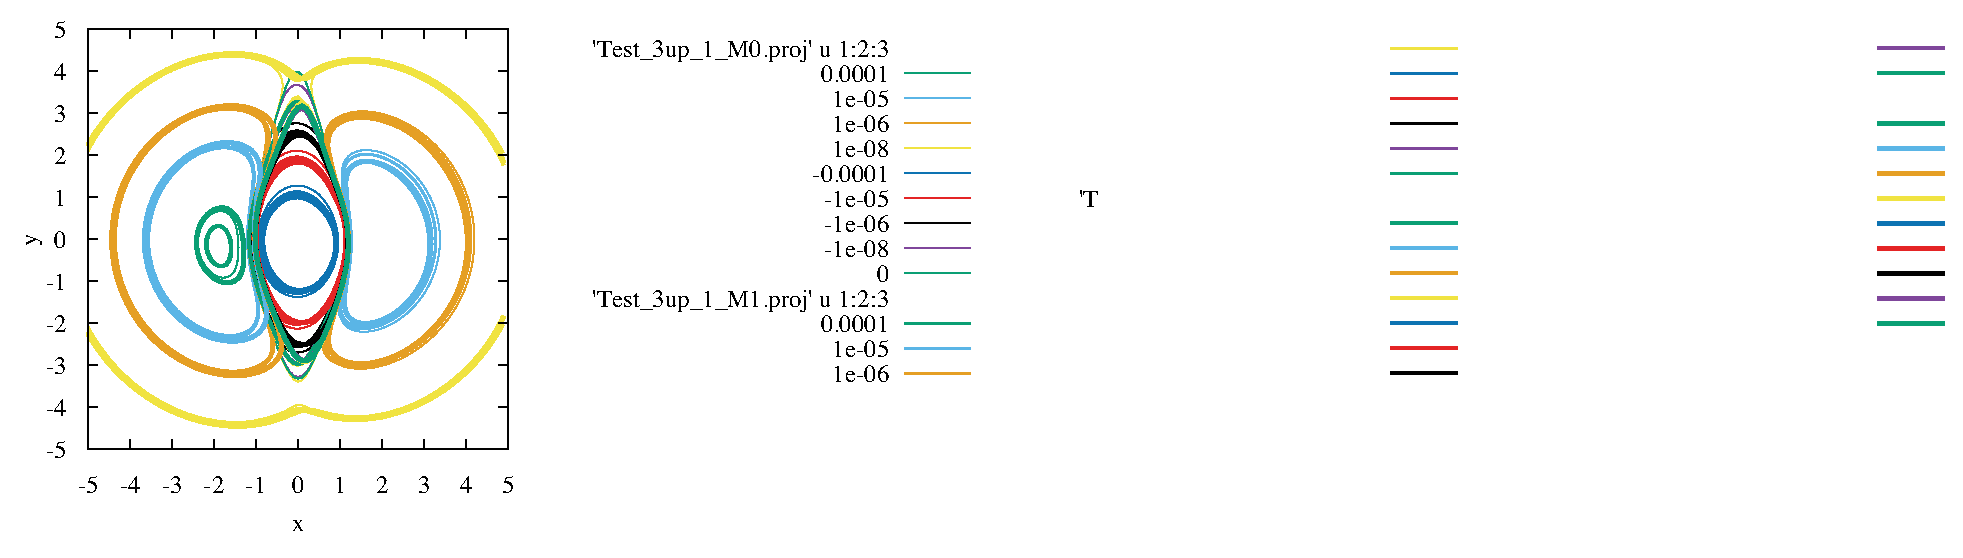
\includegraphics[scale=0.8,clip,trim=0 0 23cm 0]{Test_3up_1=1_mod}%
\caption{\label{fig:comp}
Comparison of the approximately antisymmetrized pair product projectors with the fully antisymmetrized pair product projector.
This is computed with $\tau = 1$ and three up-spin electrons.
The nucleus lies at (0, 0, 0) with $Z=2$.
The initial positions of the electrons are (-1, 0, 0), (-0.5, 0, 0), and (-1, 0, 0).
The final positions of two of the electrons are (1, 1, 1) and (-1, -1, -1).
We evaluate the projector with the final position of the other electron varying in the region $x\in[-5,5]$, $y\in[-5,5]$, and $z = 0$.
The thinest line is the exact pair product projector.
The thicker lines are the approximations.
We can see that their contours are similar.
}
\end{figure}

Finally, I have some preliminary thoughts of using random methods to approximate the permutation.
Assuming that the identity permutation has the largest contribution to the final sum.
We can start from the identity permutation and randomly swap the terms.
When the contribution drops below a certain threshold, we go back and start from the identity permutation again.
And in the end, we add up the contribution from all the unique permutations we have explored.
This may reach the desired uncertainty within a polynomial time of $N$ and is trivially parallelizable.

\subsection{Implementation}

I implement the fully antisymmetrized pair product projector and the first two approximation methods in Fortran.
The third approximation and spin treatment have also been implemented later as well by Mingtong Han and Prof. Cyrus Umrigar.
This implementation has been added into CHAMP, the QMC package we are developing.

The code starts with reading in the input file which describes the calculation to be performed.
And then it loads the corresponding pair actions that are pre-calculated with PIMC and interpolates them with a 2D cubic spline.
This includes both the electron-electron actions and the electron-nucleus actions.

Next, it calculates the pair product projector with either the fully antisymmetrized version or one of the approximations according to the command-line input.
The fully antisymmetrized method are evaluated with a recursive function.
Overall it takes $\Theta(N!)$ time and $\Theta(N)$ additional space.
The other methods use determinants to simplify the permutation calculation.
The determinants of the matrices are obtained with Gaussian elimination, which takes $\Theta(N^3)$ time.

\subsection{Stochastic Reconfiguration}

Pair product projector solves the problem of projecting onto a bosonic state.
However, it still does not solve the ``fermion sign problem'' completely.
In particular, since $\Psi_0$ and $-\Psi_0$ have the same ground state energy, walkers representing $\Psi_0$ and $-\Psi_0$ can build up and competing with each other, resulting in an extremely low signal-to-noise ratio.

Fortunately, there is an approximate method to deal with this problem, the stochastic reconfiguration method.

We define a walker to be sign violating if $\widetilde{w}_i = w_it_i/g_i < 0$.
$w_i$, $t_i$ and $g_i$ are the weight, the values of the trial and guiding wave functions respectively.
Stochastic reconfiguration tries to reconfigure the weights of all the walkers while keeping the total weights and the expectation value of a pre-selected set of observables unchanged.
Under these two constraints, we try to make the sign violation as little as possible.
A typical observable that we usually will include is the energy.

This procedure still has some bias, since the decision of what is sign violating or not at each step depends on the choice of trial wave function.
However, this bias is in our limited experience smaller than the bias introduced by the fixed-node approximation.

% If in two-column mode, this environment will change to single-column
% format so that long equations can be displayed. Use
% sparingly.
%\begin{widetext}
% put long equation here
%\end{widetext}

% figures should be put into the text as floats.
% Use the graphics or graphicx packages (distributed with LaTeX2e)
% and the \includegraphics macro defined in those packages.
% See the LaTeX Graphics Companion by Michel Goosens, Sebastian Rahtz,
% and Frank Mittelbach for instance.
%
% Here is an example of the general form of a figure:
% Fill in the caption in the braces of the \caption{} command. Put the label
% that you will use with \ref{} command in the braces of the \label{} command.
% Use the figure* environment if the figure should span across the
% entire page. There is no need to do explicit centering.



% Surround figure environment with turnpage environment for landscape
% figure
% \begin{turnpage}
% \begin{figure}
% \includegraphics{}%
% \caption{\label{}}
% \end{figure}
% \end{turnpage}

% tables should appear as floats within the text
%
% Here is an example of the general form of a table:
% Fill in the caption in the braces of the \caption{} command. Put the label
% that you will use with \ref{} command in the braces of the \label{} command.
% Insert the column specifiers (l, r, c, d, etc.) in the empty braces of the
% \begin{tabular}{} command.
% The ruledtabular enviroment adds doubled rules to table and sets a
% reasonable default table settings.
% Use the table* environment to get a full-width table in two-column
% Add \usepackage{longtable} and the longtable (or longtable*}
% environment for nicely formatted long tables. Or use the the [H]
% placement option to break a long table (with less control than
% in longtable).
% \begin{table}%[H] add [H] placement to break table across pages
% \caption{\label{}}
% \begin{ruledtabular}
% \begin{tabular}{}
% Lines of table here ending with \\
% \end{tabular}
% \end{ruledtabular}
% \end{table}

% Surround table environment with turnpage environment for landscape
% table
% \begin{turnpage}
% \begin{table}
% \caption{\label{}}
% \begin{ruledtabular}
% \begin{tabular}{}
% \end{tabular}
% \end{ruledtabular}
% \end{table}
% \end{turnpage}

% Specify following sections are appendices. Use \appendix* if there
% only one appendix.
%\appendix
%\section{}

% If you have acknowledgments, this puts in the proper section head.
\section{}
\section{Acknowledgments}
\begin{acknowledgments}
I gratefully thank Cyrus Umrigar for helping me understand quantum Monte Carlo and leading me to this problem.
I also gratefully thank all the other group members, including Mingtong Han, Matthew Otten, and Adam Holmes for the useful discussions and patient help.
\end{acknowledgments}

% Create the reference section using BibTeX:
\nocite{*}
\bibliography{ppp}

\end{document}
%
% ****** End of file apstemplate.tex ******

%
% \begin{table}%[H] add [H] placement to break table across pages
% \caption{\label{tab:compare} Cohesive energy of Si obtained through various computational methods and compared with experimental values.}
% \begin{ruledtabular}
% \begin{tabular}{l | c c c c}
% Method & DFT & VMC & DMC & Experiment \\
% \hline
% Energy (\electronvolt) & 5.28\footnotemark[1] & 4.48(1)\footnotemark[2] & 4.63(2)\footnotemark[2] & 4.62(8)\footnotemark[1] \\
% \end{tabular}
% \end{ruledtabular}
% \footnotetext[1]{Farid and Needs}
% \footnotetext[2]{Leung \emph{et~al.}}
% \end{table}
